\documentclass[9pt,a4paper]{extarticle}
\usepackage[left=1.45cm,right=1.45cm,top=1.55cm,bottom=1.45cm]{geometry}
\usepackage[T1]{fontenc}
\usepackage[utf8]{inputenc}
% Latin Modern is the traditional Computer Modern design used in scientific LaTeX.
% The equations below also use only KaTeX-supported commands.
\usepackage{lmodern}
\usepackage{amsmath,amssymb}
\usepackage{siunitx}
\usepackage{microtype}
\usepackage{graphicx,tabularx,array,xcolor,booktabs,fancyhdr,hyperref,textcomp}
\usepackage{caption,float}
\usepackage[compact]{titlesec}
\usepackage{enumitem}
\usepackage{pgfplots}
\pgfplotsset{compat=1.18}
\definecolor{SPHEREblue}{HTML}{203864}
\hypersetup{colorlinks=true,linkcolor=SPHEREblue,urlcolor=SPHEREblue}
\pagestyle{fancy}\fancyhf{}
\lhead{\footnotesize SPHERE | Human Spaceflight Technology | Team Engineering Report}
\rfoot{\footnotesize Page \thepage}
\fancypagestyle{plain}{%
  \fancyhf{}%
  \lhead{\footnotesize SPHERE | Human Spaceflight Technology | Team Engineering Report}%
  \rfoot{\footnotesize Page \thepage}%
}
\setlength{\parindent}{1em}
\setlength{\parskip}{1.5pt}
\setlength{\headheight}{14pt}
\setlength{\columnsep}{0.65cm}
\setlength{\columnseprule}{0.15pt}
\setlength{\tabcolsep}{2.5pt}
\setlength{\emergencystretch}{1em}
\renewcommand{\arraystretch}{1.10}
\titlespacing*{\section}{0pt}{6pt}{3pt}
\titlespacing*{\subsection}{0pt}{4pt}{2pt}
\setlist{nosep,leftmargin=*}
\sisetup{detect-all,per-mode=symbol,range-phrase=--,range-units=single}
\newcommand{\Tenv}{T_{\mathrm{env}}}
\newcommand{\Tzero}{T_{0}}
\newcommand{\MLI}{\textsc{mli}}
\newcommand{\EUR}[1]{\texteuro\,#1}
\begin{document}
\twocolumn[{
\begin{center}
{\LARGE\bfseries SPACESUIT THERMAL SHIELDING KIT\par}
\vspace{1mm}{\Large\color{SPHEREblue} Team Engineering Report\par}\vspace{3mm}
{\small Human Spaceflight Technology, TUM School of Engineering and Design\par}
{\small Piyath Vithanage \,\textperiodcentered\, Elio Krollpfeiffer \,\textperiodcentered\, Dilan Fernando \,\textperiodcentered\, Nuhansee Migelhewage\par}
{\small 17 September 2026\par}
\end{center}
\vspace{2mm}
\begin{minipage}{0.92\textwidth}\small
\textbf{Abstract---}SPHERE is a reusable classroom experiment for studying transient heat transfer. Students compare four insulation configurations by cooling matched \SI{100}{\milli\litre} water capsules in an ice-water bath. Mission Control calculates a Newtonian-cooling prediction, records sixteen manual temperature readings and plots the measured and predicted curves together. The worked dataset ranks the full multilayer package first and demonstrates why a reflective layer must be evaluated in its actual boundary condition. This report documents the learning design, apparatus, model, method, software, safety, budget evidence and limitations.
\end{minipage}
\vspace{4mm}
}]
\subsection*{Executive summary}
In the worked dataset, the full multilayer package produced the smallest temperature drop, followed by bubble wrap. Mylar alone did not perform as predicted. This is consistent with the test boundary: the water bath strongly promotes conduction and convection, while reflective foil is mainly used to reduce radiative transfer. The experiment should therefore be treated as a classroom model of thermal-control principles rather than as a vacuum simulation or an aerospace qualification test.

The team report is limited to ten pages. It is followed by one contribution statement from each team member, as required in the project brief.

\subsection*{Key project settings}
Matched \SI{100}{\milli\litre} cores; an initial temperature of approximately \SI{80}{\celsius}; a measured ice-water boundary; one reading per minute from \SIrange{0}{15}{\minute}; bare, bubble-wrap, Mylar-only and full multilayer conditions; and analysis using temperature drop, residuals, mean absolute error and the effective cooling coefficient $k$.

\section*{1 Project purpose and learning design}
\subsection*{1.1 Educational objective}
The project turns the problem of spacesuit thermal protection into an experiment that can be completed during a double lesson. Students distinguish conduction, convection and radiation, apply Newton's cooling model, record a controlled temperature series and explain why the measured curve differs from the prediction.

The learning sequence mirrors an engineering test campaign: define a requirement, choose a configuration, commit to a prediction, assemble the test article, control variables, collect telemetry and evaluate the evidence. The spacesuit context motivates the exercise, while the teacher explicitly states where the analogy ends. In vacuum, external convection is absent and radiation is important; in the classroom bath, liquid contact and convection dominate.

\subsection*{1.2 Classroom workflow}
Four groups work in parallel, with one insulation condition assigned to each group. A complete session takes approximately \SIrange{55}{70}{\minute}, including the briefing, safety check, assembly, a \SI{15}{\minute} measurement period and the final analysis. The website runs in a standard browser and does not require a user account, native application or wireless sensor connection.

\subsection*{1.3 Success criteria}
A successful run contains all sixteen time-temperature points or documents missing readings; records the actual start and bath temperatures; uses matched geometry, water volume, probe depth and immersion depth; documents layer order and wetting; and reports both the observed ranking and the limitations of that comparison.

\begin{center}\small
\begin{tabularx}{\columnwidth}{|>{\raggedright\arraybackslash}X|>{\raggedright\arraybackslash}X|>{\raggedright\arraybackslash}X|}\hline
\textbf{Requirement} & \textbf{Implementation} & \textbf{Evidence} \\ \hline
Engaging & Spacesuit narrative and four-way comparison & Prediction, physical build and visible curves \\ \hline
Reusable & Matched jars, probes and removable wraps & Repeated classroom use \\ \hline
Safe & Adult hot-water handling and stop criteria & Risk controls in Section 6 \\ \hline
Assessable & Residuals, MAE and written interpretation & Worksheet and ten-question assessment \\ \hline
\end{tabularx}
\end{center}
\section*{2 Thermodynamic framework and insulation design}
\subsection*{2.1 Reference model}
The water is treated as a lumped thermal mass, so its temperature is assumed to be spatially uniform at each measurement time. The reference curve is
\begin{equation}
  T(t)=T_{\mathrm{env}}+\left(T_0-T_{\mathrm{env}}\right)e^{-kt},
  \label{eq:newton}
\end{equation}
where $\Tzero$ is the measured initial temperature, $\Tenv$ is the measured bath temperature and $k$ is an effective cooling coefficient in \si{\per\minute}. The value of $k$ represents the complete assembled system, including geometry, thermal mass, boundary conditions and all active heat-transfer paths. It is not the thermal conductivity of an individual material. A smaller $k$ indicates slower cooling under otherwise comparable conditions.

The sensible-energy change is estimated from
\begin{equation}
  \Delta Q = m c_p \Delta T.
  \label{eq:energy}
\end{equation}
For \SI{100}{\milli\litre} of water, $m\approx\SI{0.10}{\kilogram}$. Taking $c_p\approx\SI{4184}{\joule\per\kilogram\per\kelvin}$, a \SI{10}{\kelvin} temperature drop corresponds to approximately \SI{4.18}{\kilo\joule} leaving the water. This is only an estimate because the jar, probe and insulation also store energy and the water may not remain perfectly mixed.

\subsection*{2.2 Layer strategy}
The bare jar establishes the baseline. Bubble wrap traps air and interrupts conductive and convective paths. A single Mylar layer chiefly changes radiative exchange and provides little protection against direct liquid contact. The full package places cotton against the jar, bubble wrap in the middle and Mylar outside. Layers are secured without compression because trapped air is part of the thermal resistance.

\begin{figure}[H]\centering
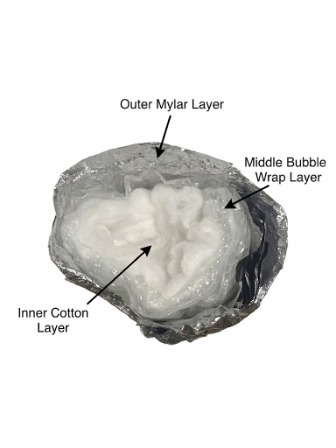
\includegraphics[width=\columnwidth,height=4.2cm,keepaspectratio]{latex_assets/figure2_cross_section.jpg}
\caption*{\small Figure 2. Cross-section of the full multilayer package: cotton, bubble wrap and outer Mylar.}
\end{figure}
\begin{center}\small
\begin{tabularx}{\columnwidth}{|>{\raggedright\arraybackslash}X|>{\raggedright\arraybackslash}X|>{\raggedright\arraybackslash}X|}\hline
\textbf{Condition} & \textbf{Construction} & \textbf{Reference $k$ (\si{\per\minute})} \\ \hline
Bare & Uninsulated matched core & 0.150 \\ \hline
Bubble wrap & Two uncompressed layers & 0.040 \\ \hline
Mylar only & One reflective layer; neck closed & 0.121 \\ \hline
Full MLI & Cotton + bubble wrap + Mylar & 0.015 \\ \hline
\end{tabularx}
\end{center}
\section*{3 Hardware and experimental method}
\subsection*{3.1 Apparatus}
The apparatus comprises four matched \SI{100}{\milli\litre} heat-safe cores, four core thermometers, a separate bath thermometer, a stable bath container, a timer, cotton, bubble wrap, Mylar and reusable fastening material. Each probe is centred in the water and supported by the closure. The display and cable connection remain outside the bath.

\subsection*{3.2 Procedure}
\begin{enumerate}
  \item Prepare a stable, dry work area and separate all electronics from the water.
  \item Measure and record $\Tenv$.
  \item Fill each core with \SI{100}{\milli\litre} of water near \SI{80}{\celsius} and record $\Tzero$.
  \item Centre the probe and leak-test the closure.
  \item Apply the assigned insulation without compressing the cotton or bubble wrap.
  \item Immerse the core and start the timer immediately.
  \item Record one temperature reading per minute until $t=\SI{15}{\minute}$.
  \item Calculate the temperature drop, residuals, MAE and an effective value of $k$.
\end{enumerate}

If starting temperatures differ, configurations are compared by temperature drop, the dimensionless ratio $\theta=(T-T_{\mathrm{env}})/(T_0-T_{\mathrm{env}})$, or a fitted value of $k$ rather than final temperature alone. Actual timestamps are used for late readings. The bath is checked again when ice visibly melts. Any classroom percentage referenced to \SI{20}{\celsius} is labelled separately and is not mixed with this bath-referenced quantity.

\subsection*{3.3 Fair-test controls}
Jar geometry, fill mass, probe depth, immersion depth, sampling interval and bath position are held constant. Photographs or written notes record layer order, gaps, compression, leakage and wetting. A run is rejected when containment or measurement integrity is lost.

\begin{figure}[H]\centering
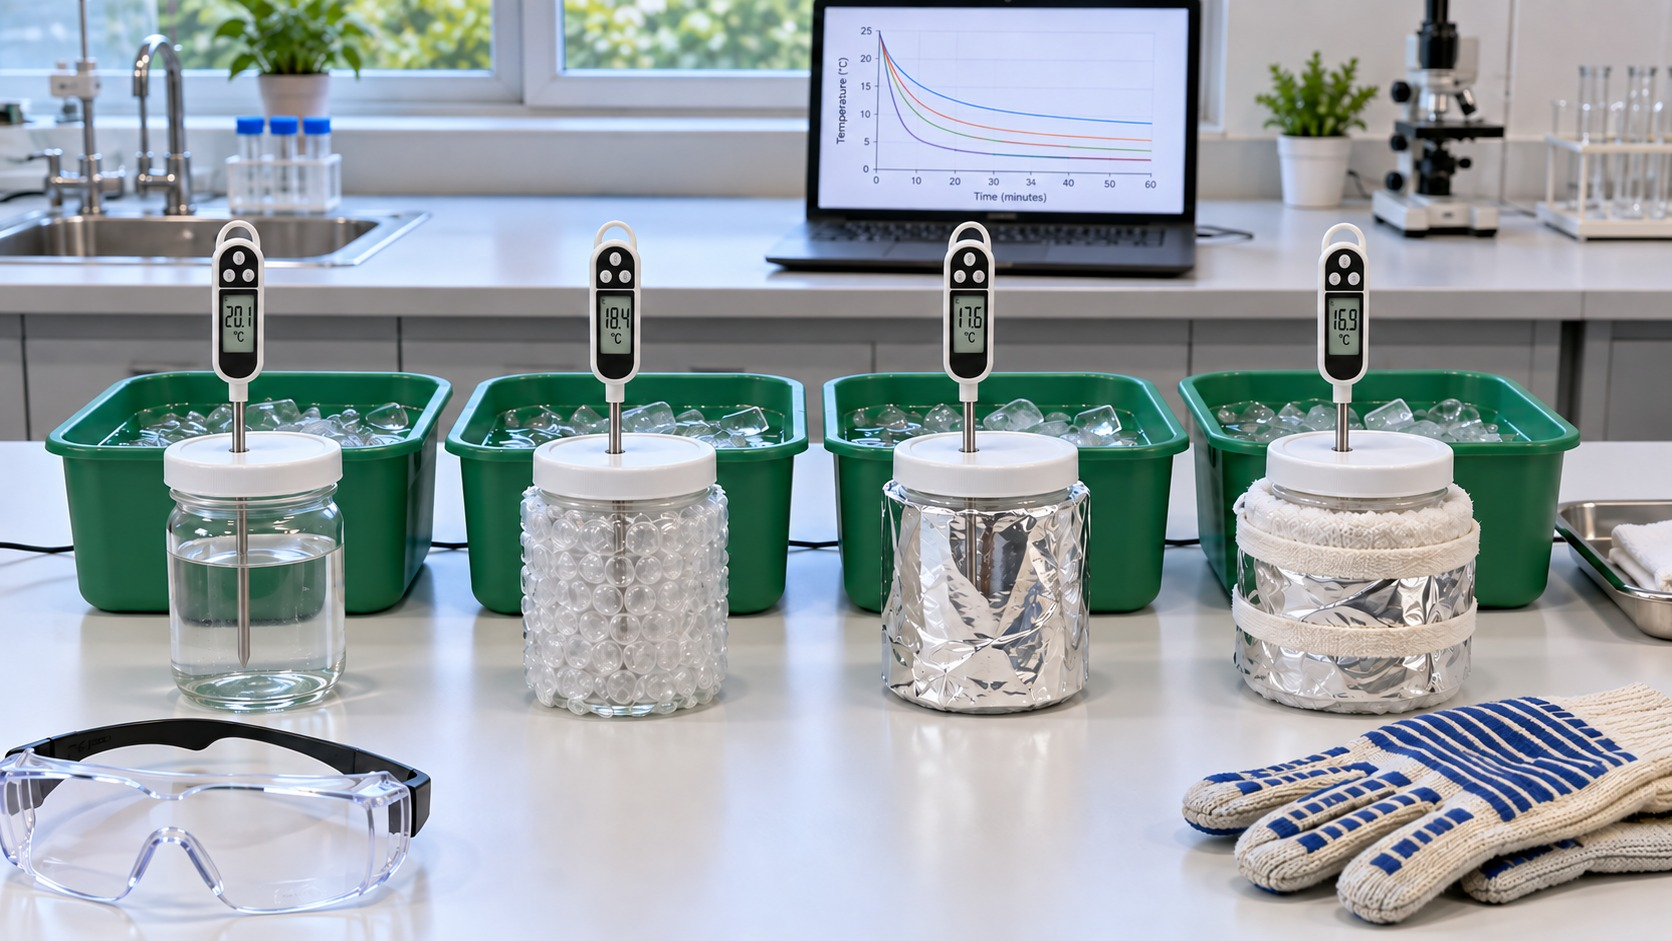
\includegraphics[width=\columnwidth,height=4.2cm,keepaspectratio]{latex_assets/figure7_configurations.jpg}
\caption*{\small Figure 7. Four physical configurations prepared for comparative testing.}
\end{figure}
\section*{4 Mission Control and data workflow}
\subsection*{4.1 Software role}
Mission Control is a static HTML, CSS and JavaScript application hosted at \url{https://hsp-mc.github.io/}. Students select a configuration, enter $\Tzero$ and $\Tenv$, generate a reference curve and manually enter the measured temperatures. Chart.js plots the series and KaTeX renders the equations. Browser storage protects an active session from an accidental refresh. A three-question pre-flight gate, study flashcards, a timed ten-question quiz and a leaderboard support assessment. Leaderboard synchronization through Supabase is optional, and a local fallback remains available. Experimental telemetry is not uploaded as a permanent project database.

\subsection*{4.2 Prediction to evaluation}
The workflow has four stages. First, the prediction is calculated from $\Tzero$, $\Tenv$, $k$ and the selected duration. The acquisition stage runs the timer and stores the sixteen-point log. The comparison view overlays the measured and predicted curves and lists their signed residuals. Finally, the evaluation view reports the mean absolute error and asks students to discuss the cause of the disagreement.

Manual entry is intentional. It avoids pairing and sensor-interface failures while keeping students responsible for each observation. A print view preserves the settings and telemetry for a worksheet. The instructor gate is only a classroom convenience and is not presented as a security boundary.

\subsection*{4.3 Reliability and offline use}
The core application needs no database or server runtime. For fully offline delivery, Chart.js, KaTeX, Lucide and fonts should be bundled locally. The printed procedure and task sheet provide an analog fallback when a school cannot depend on internet access or student devices.

\begin{figure}[H]\centering
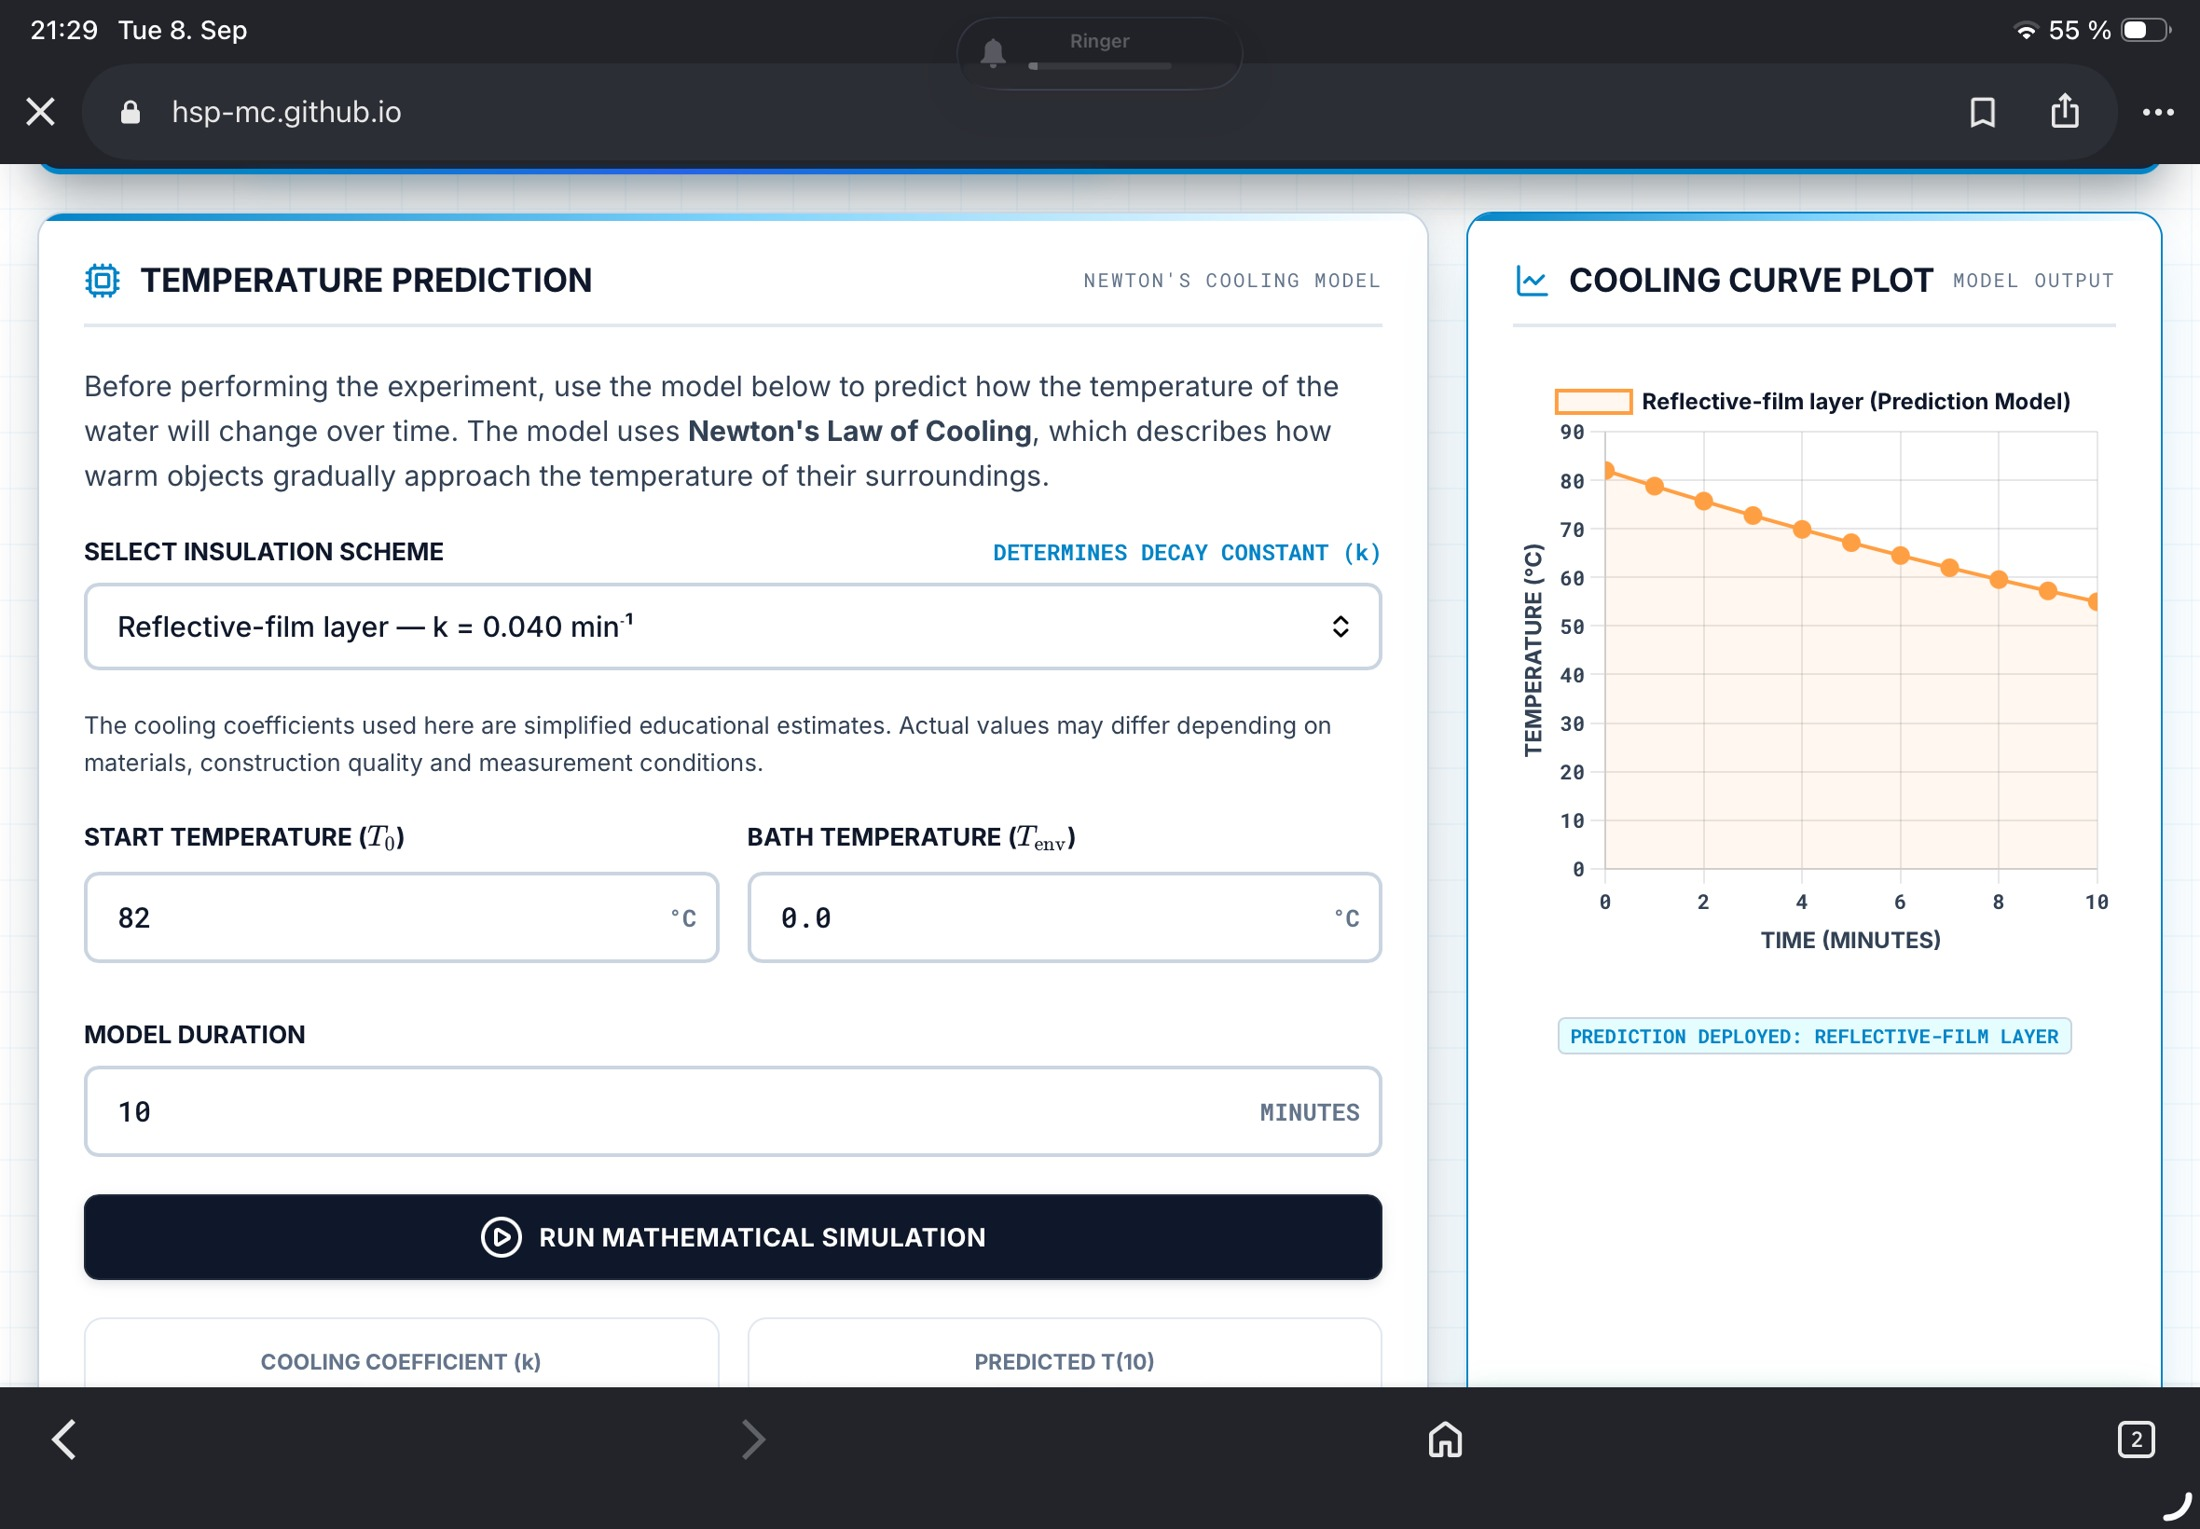
\includegraphics[width=\columnwidth,height=4.2cm,keepaspectratio]{latex_assets/figure8_mission_control.jpg}
\caption*{\small Figure 8. Mission Control prediction interface with model inputs and cooling curve.}
\end{figure}
\section*{5 Worked results and model comparison}
\subsection*{5.1 Observed ranking}
The supplied worked example gives the smallest temperature drop for the full multilayer package (\SI{14.9}{\celsius}), followed by bubble wrap (\SI{30.0}{\celsius}). The bare control dropped by \SI{44.9}{\celsius}, while the Mylar-only condition dropped by \SI{47.2}{\celsius}. Because $\Tzero$ differed among runs, final temperature alone is not a fair ranking measure. Temperature drop, bath-referenced $\theta$ and a fitted value of $k$ are more appropriate for this comparison.

\subsection*{5.2 Model agreement}
Dashboard scores were \SI{93}{\percent} for full MLI, \SI{83}{\percent} for bubble wrap, \SI{94}{\percent} for the bare control and \SI{3}{\percent} for Mylar only. The low Mylar score indicates a large mismatch between the reference curve and the assembled test article. Possible causes include liquid contact at the neck, an absent air gap, probe variation or a reference value of $k$ that did not represent the actual build.

These data support a classroom worked example, not a general material certification. Repeated trials with calibrated probes are required before reporting uncertainty or population-level differences.

\begin{figure}[H]\centering
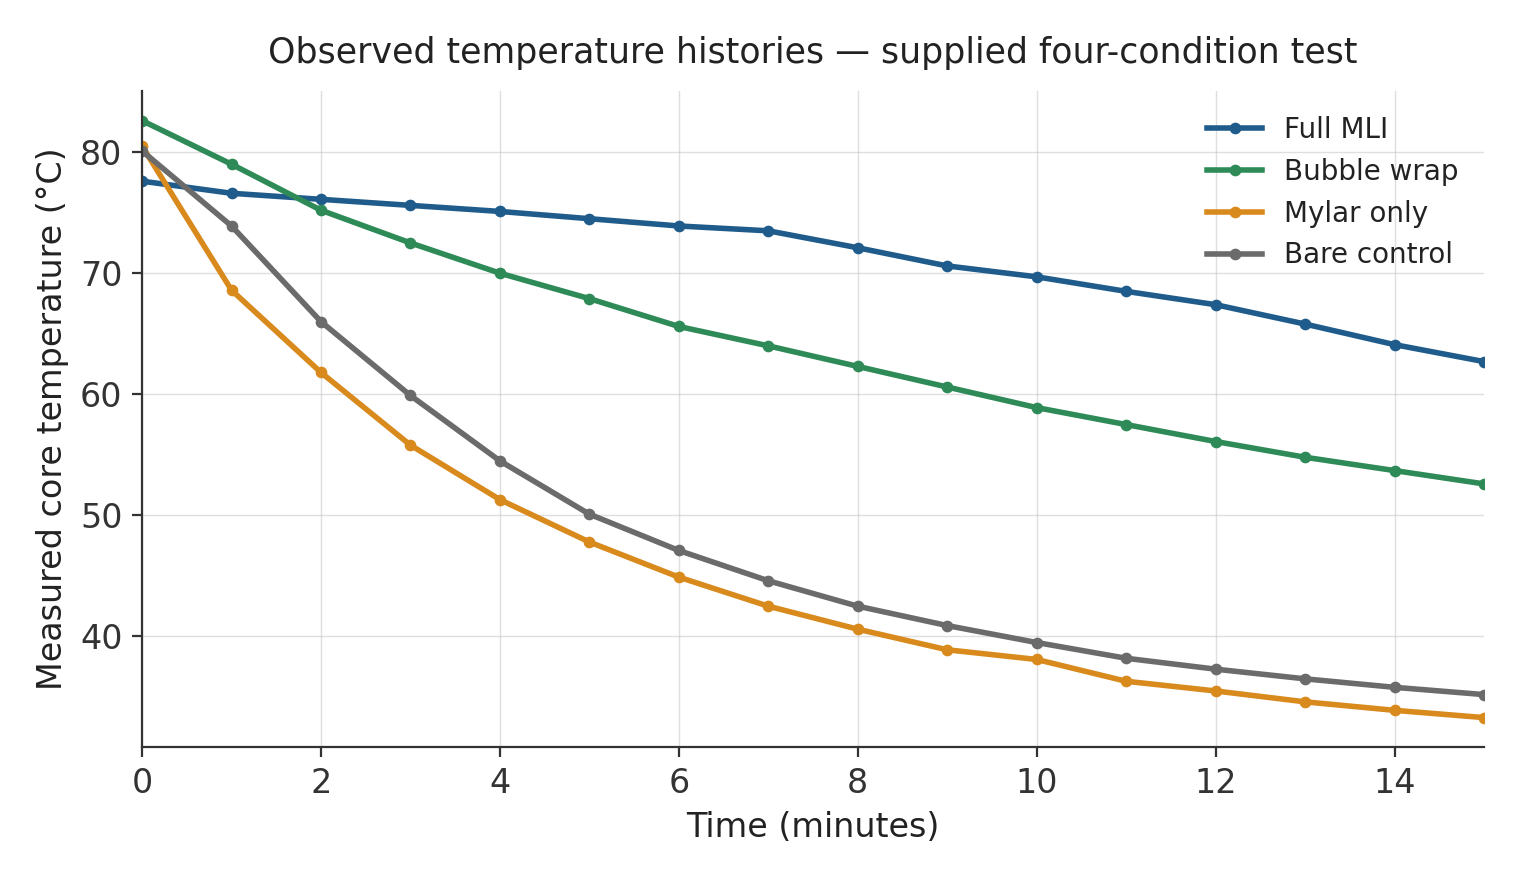
\includegraphics[width=\columnwidth,height=4.2cm,keepaspectratio]{latex_assets/figure11_results.png}
\caption*{\small Figure 11. Observed temperature histories for the supplied four-condition worked example.}
\end{figure}
\begin{center}\small
\begin{tabularx}{\columnwidth}{|>{\raggedright\arraybackslash}X|>{\raggedright\arraybackslash}X|>{\raggedright\arraybackslash}X|>{\raggedright\arraybackslash}X|>{\raggedright\arraybackslash}X|}\hline
\textbf{Condition} & \textbf{T0} & \textbf{T15} & \textbf{Drop} & \textbf{Score} \\ \hline
Full MLI & \SI{77.6}{\celsius} & \SI{62.7}{\celsius} & \SI{14.9}{\celsius} & \SI{93}{\percent} \\ \hline
Bubble wrap & \SI{82.6}{\celsius} & \SI{52.6}{\celsius} & \SI{30.0}{\celsius} & \SI{83}{\percent} \\ \hline
Bare & \SI{80.1}{\celsius} & \SI{35.2}{\celsius} & \SI{44.9}{\celsius} & \SI{94}{\percent} \\ \hline
Mylar only & \SI{80.5}{\celsius} & \SI{33.3}{\celsius} & \SI{47.2}{\celsius} & \SI{3}{\percent} \\ \hline
\end{tabularx}
\end{center}
\section*{6 Uncertainty, safety and risk controls}
\subsection*{6.1 Measurement uncertainty}
The residual at each measurement time and the mean absolute error are defined as
\begin{align}
  r_i &= T_{\mathrm{measured},i}-T_{\mathrm{model},i},\\
  \mathrm{MAE} &= \frac{1}{n}\sum_{i=1}^{n}\lvert r_i\rvert.
\end{align}
These quantities describe the size of the model disagreement but do not identify its physical cause. The main uncertainty sources are probe contact with the jar wall, leakage at the neck, thermal stratification, bath warming, unequal immersion depth, different starting conditions, varying wrap area and layer compression. The lumped model also assumes a uniform core temperature and a constant effective $k$.

\subsection*{6.2 Mandatory controls}
An instructor handles the water near \SI{80}{\celsius}; boiling water is not used. Eye protection and heat-resistant gloves or tongs are required. The bath is kept stable, below waist height and separated from electronic devices. Only undamaged heat-safe containers are used, closures are leak-tested, and displays and connectors remain dry. The run stops immediately if the container leaks, the probe moves, the insulation becomes wet or the initial temperature is outside the agreed range.

\subsection*{6.3 Risk assessment}
The dominant hazard is scalding during filling and transfer. Administrative controls assign hot-water handling to an adult and keep the hot zone separate from data-entry devices. Engineering controls include secondary containment, supported probes and low-voltage thermometers. Continuing a leaking run would create both an unsafe condition and invalid data, so the stop rule is absolute.

\subsection*{6.4 Recommended validation}
Repeat every condition at least three times; randomize run order; weigh the water; photograph probe depth and closure; record actual bath temperature; and fit k from all valid points rather than a single endpoint. Report variability across repeats.

\begin{center}\small
\begin{tabularx}{\columnwidth}{|>{\raggedright\arraybackslash}X|>{\raggedright\arraybackslash}X|>{\raggedright\arraybackslash}X|}\hline
\textbf{Hazard or failure} & \textbf{Control} & \textbf{Stop criterion} \\ \hline
Scalding & Adult handling; PPE; stable bath & Spill or unstable vessel \\ \hline
Water/electronics & Dry-zone separation & Wet display or connector \\ \hline
Loss of containment & Pre-test leak check & Leak or wet insulation \\ \hline
Invalid measurement & Centred supported probe & Probe shift or invalid $T_0$ \\ \hline
\end{tabularx}
\end{center}
\section*{7 Budget, feasibility and classroom package}
\subsection*{7.1 Documented budgeting}
The kickoff brief set an affordability target of approximately \EUR{50}. The project draft allocates \EUR{11} to four \SI{100}{\milli\litre} jars with cable glands, \EUR{16} to four digital probe thermometers, \EUR{8} to the insulation materials and \EUR{5} to the test tub. The resulting planning total is \EUR{40}. These are item-level engineering estimates rather than final invoiced prices; the final bill of materials should be updated from receipts before the kit is reproduced.

\subsection*{7.2 Reusability and operating cost}
Jars, probes, bath container and fasteners are reusable. Cotton, bubble wrap and Mylar can also be reused when kept dry and uncompressed. The software has no license fee and runs in an ordinary browser. Schools should re-quote locally and record quantities, shipping and substitutions before adoption.

\subsection*{7.3 Delivered learning package}
The kit is accompanied by student and teacher manuals, an illustrated procedure, a task sheet, revision flashcards, Mission Control and an aligned assessment. All materials use the same variables, settings and four configurations. This consistency reduces setup errors and lets teachers move between explanation, test and assessment without translating terminology.

\begin{figure}[H]\centering
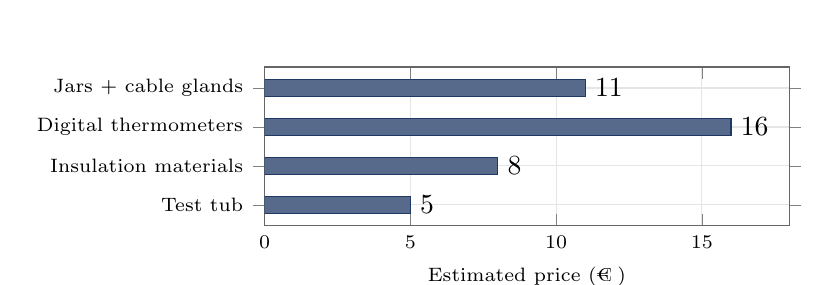
\begin{tikzpicture}
\begin{axis}[
  xbar, width=0.68\columnwidth, height=3.6cm,
  xmin=0, xmax=18,
  xlabel={Estimated price (\EUR{})},
  symbolic y coords={Test tub,Insulation materials,Digital thermometers,Jars + cable glands},
  ytick=data, nodes near coords,
  nodes near coords align={horizontal},
  bar width=6pt,
  tick label style={font=\scriptsize},
  label style={font=\scriptsize},
  axis line style={draw=black!60},
  grid=major, grid style={black!10},
  enlarge y limits=0.18]
\addplot[fill=SPHEREblue!75,draw=SPHEREblue] coordinates {(5,Test tub) (8,Insulation materials) (16,Digital thermometers) (11,Jars + cable glands)};
\end{axis}
\end{tikzpicture}
\caption*{\small Item estimates total \EUR{40}, below the \EUR{50} target.}
\end{figure}
\section*{8 Educational delivery and conclusions}
\subsection*{8.1 Student and teacher use}
Students predict the ranking, build one condition, collect readings, calculate error and explain why the model and experiment differ. Teachers receive timing, safety guidance, discussion prompts and assessment criteria. Inquiry prompts such as ``What happens if the wrap is compressed?'' or ``How does a warmer bath change the curve?'' support design iteration without changing the core procedure.

\subsection*{8.2 Main engineering conclusion}
SPHERE closes a complete theory-to-evidence loop with accessible hardware. In the worked example, full MLI performed best and bubble wrap second. The weak Mylar-only result is pedagogically valuable because it shows that a good material for one transfer mechanism can perform poorly when another mechanism dominates. The correct conclusion is conditional on the water-bath boundary and construction quality.

\subsection*{8.3 Next steps}
The next test campaign should add replicate runs, randomized order, calibrated probes, measured water mass and run metadata. Mission Control should add CSV export and an offline asset bundle. The team should also retain a one-page equipment checklist and a receipt-based bill of materials for future classroom deployment.

\subsection*{8.4 Scope statement}
The kit is suitable for comparative classroom teaching when the stated controls are used. It is not a vacuum simulation and does not certify any material for aerospace, pressure-vessel, fire-protection or personal-protective use.

\begin{figure}[H]\centering
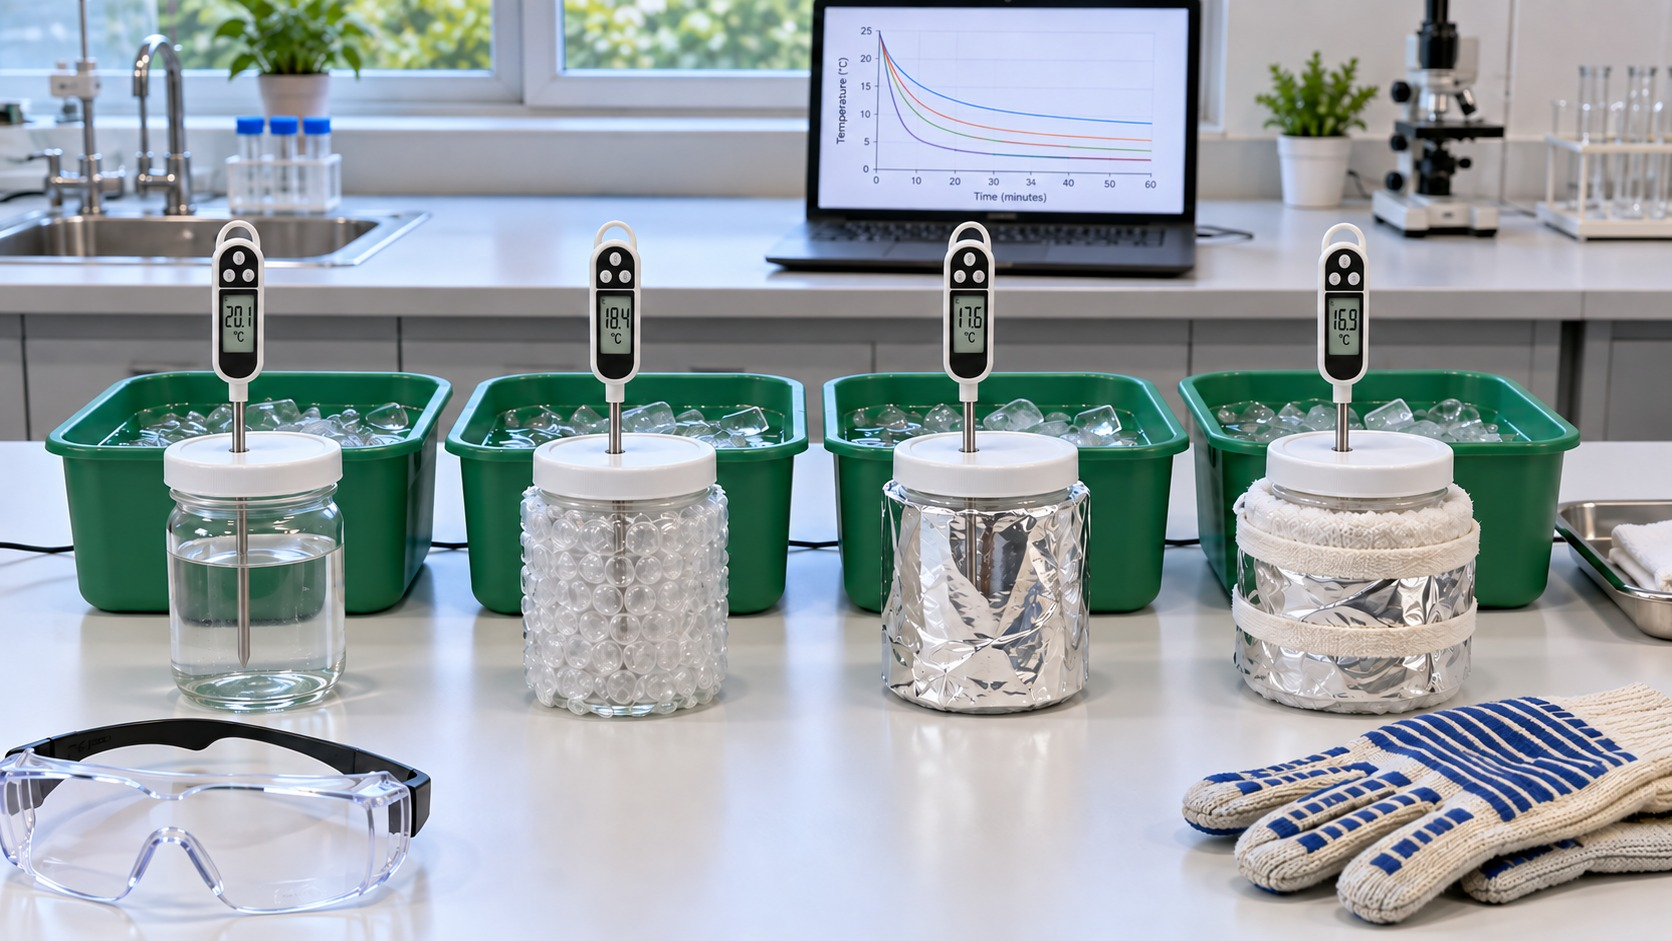
\includegraphics[width=\columnwidth,height=4.2cm,keepaspectratio]{latex_assets/figure13_complete_system.jpg}
\caption*{\small Figure 13. Complete classroom system with four test articles and the digital interface.}
\end{figure}
\section*{9 Project cross-reference, references and responsibilities}
\subsection*{9.1 Cross-reference audit}
The report was checked against the live Mission Control site, its source files, the student and teacher manuals, task sheet, flashcards, procedure, project draft and presenter guide. The current controlled values are the website/manual coefficients (bare 0.150, bubble wrap 0.040, Mylar 0.121 and full MLI 0.015~\si{\per\minute}), a \SI{15}{\minute} run with sixteen readings, and the four-condition build described here. Earlier draft wording that assigns 0.040~\si{\per\minute} to Mylar or alternates between PET and glass without recording the actual vessel is superseded by this configuration-controlled description.

\begin{center}\scriptsize
\begin{tabularx}{\columnwidth}{@{}>{\raggedright\arraybackslash}p{0.26\columnwidth}>{\raggedright\arraybackslash}X>{\raggedright\arraybackslash}p{0.18\columnwidth}@{}}
\toprule
\textbf{Report element} & \textbf{Project evidence} & \textbf{Status} \\
\midrule
Model and constants & Live site, \texttt{app.js}, manuals & Aligned \\
Method and safety & Manuals, task sheet, procedure & Aligned \\
Results and MAE & Project telemetry and website workflow & Aligned \\
Assessment & Pre-flight gate, flashcards, ten-question quiz & Aligned \\
Budget & Item estimate in project draft & Estimate \\
Validation & One worked series per condition & Partial \\
\bottomrule
\end{tabularx}
\end{center}

The submission report is complete against the kickoff headings. Engineering validation remains incomplete until replicated trials, calibrated uncertainty estimates and final receipt-based costs are available; these limitations are stated rather than filled with unsupported claims.

\subsection*{9.2 References}
\begingroup
\small
\sloppy
\setlength{\itemsep}{1pt}
\begin{thebibliography}{9}
\bibitem{nasa-suit} NASA Johnson Space Center, ``Spacewalk Spacesuit Basics.'' Available: \url{https://www.nasa.gov/centers-and-facilities/johnson/spacewalk-spacesuit-basics/}. Accessed 9 September 2026.
\bibitem{nist-water} National Institute of Standards and Technology, ``Water, Liquid Phase Heat Capacity,'' \emph{NIST Chemistry WebBook}, SRD 69. Available: \url{https://webbook.nist.gov/cgi/cbook.cgi?ID=C7732185&Table=on&Type=JANAFL}. Accessed 9 September 2026.
\bibitem{mli-guide} M. M. Finckenor and D. Dooling, \emph{Multilayer Insulation Material Guidelines}, NASA/TP-1999-209263, 1999.
\bibitem{thermal-guide} NASA, \emph{Passive Thermal Control Engineering Guidebook}, Rev. 4.0, 2023.
\bibitem{chartjs} Chart.js Contributors, ``Chart.js Documentation.'' Available: \url{https://www.chartjs.org/docs/latest/}. Accessed 9 September 2026.
\bibitem{katex} Khan Academy and KaTeX Contributors, ``KaTeX Documentation.'' Available: \url{https://katex.org/docs/}. Accessed 9 September 2026.
\bibitem{mission-control} SPHERE Project Team, ``Mission Control.'' Available: \url{https://hsp-mc.github.io/}. Accessed 9 September 2026.
\bibitem{kickoff} Human Spaceflight Technology, \emph{Engineering Project Kick-Off}, TUM School of Engineering and Design, 5 May 2026.
\bibitem{project-materials} SPHERE Project Team, student manual, teacher manual, task sheet, flashcards, illustrated procedure and project telemetry, 2026.
\end{thebibliography}
\endgroup

\subsection*{9.3 Report structure}
The team engineering report ends on this page and remains within the ten-page limit. Four one-page individual contribution statements follow. Figure numbering is retained from the established project record; the opening figure from the earlier draft is not included.

\begin{center}\small
\begin{tabularx}{\columnwidth}{|>{\raggedright\arraybackslash}X|>{\raggedright\arraybackslash}X|}\hline
\textbf{Member} & \textbf{Documented primary responsibility} \\ \hline
Piyath Vithanage & Current application, telemetry, graphs, quiz, leaderboard, resources and integration \\ \hline
Dilan Fernando & Thermodynamic model, physical test system, analysis, technical writing and integration \\ \hline
Elio Krollpfeiffer & Early website development, styling, student and teacher manuals, and media assets \\ \hline
Nuhansee Migelhewage & Heat-transfer theory, experimental setup, practical preparation and results presentation \\ \hline
\end{tabularx}
\end{center}
\clearpage
\onecolumn
\fontsize{12}{18}\selectfont
\setlength{\parskip}{4pt}
\section*{Individual contribution -- Piyath Vithanage}
\subsection*{Role and completed work}
My main contribution was the current Mission Control application and the integration of the final project resources. I developed the browser workflow that connects the briefing, assembly instructions, prediction, measurement, study material and assessment. I used HTML for the experiment structure, CSS for the responsive interface and JavaScript for the model, timer, telemetry, quiz and leaderboard behaviour.

I connected the configuration selector, starting temperature, bath temperature, duration and cooling coefficient to one application state. I implemented the \SI{15}{\minute} timer and manual telemetry workflow. The page validates entries, stores the active model and data in the browser, overlays measured and predicted curves, calculates MAE and produces a printable telemetry record.

\subsection*{Graphing and analysis}
I developed the graphing workflow so that students can compare the measured and predicted temperatures on the same time axis. I kept the configuration names and colours consistent across the selector, summary, graph and results table. I also implemented the residual and MAE calculations. These outputs make the graph part of the analysis rather than only a visual display.

The implementation keeps calculated and measured data as separate series and restores the current session from local browser storage. Defensive checks around optional interface elements prevent one missing panel from stopping the simulator. The print view records the selected configuration, model settings, chart, measurement count and error result in a form that can be attached to the task sheet.

\subsection*{Assessment and integration}
I developed the timed ten-question classroom challenge, answer review, scoring, winner presentation and leaderboard. The leaderboard stores results locally by default and can synchronize across devices through the optional Supabase configuration. I also aligned the student manual, teacher manual, task sheet, flashcards, presentation material and README with the current experiment and website.

The final integration included checking the same question topics across online and printable resources, preserving mathematical notation through KaTeX, and maintaining a usable layout on desktop and mobile screens. The thermal model and telemetry remain local to the browser when the optional shared leaderboard is unavailable.

\begin{center}\small
\begin{tabularx}{0.86\textwidth}{@{}>{\bfseries}p{0.26\textwidth}X@{}}
\toprule
Deliverable & Evidence \\
\midrule
Application workflow & \texttt{index.html}, \texttt{app.js} and \texttt{styles.css} \\
Prediction and telemetry & Model, timer, chart, MAE and print functions \\
Assessment & Timed quiz, answer review, scoring and leaderboard \\
Resource integration & Manuals, task sheet, flashcards, README and presentation \\
\bottomrule
\end{tabularx}
\end{center}

My next improvement would be CSV export with run metadata and a packaged offline build. These changes would improve reproducibility without adding sensor complexity.

\clearpage
\section*{Individual contribution -- Dilan Fernando}
\subsection*{Role and completed work}
My main technical responsibility was the thermodynamic definition of the experiment and interpretation of the physical results. I selected the lumped Newtonian cooling model because it gives students a manageable equation while preserving the relationship between thermal mass, environmental temperature and cooling rate. I defined $k$ as an effective system coefficient in \si{\per\minute} and kept it separate from material thermal conductivity.

I established the final test conditions: a \SI{100}{\milli\litre} water core, a starting temperature near \SI{80}{\celsius}, a measured ice-water bath and one reading per minute for \SI{15}{\minute}. I linked those settings to the apparatus and procedure so that the model and physical experiment describe the same system.

\subsection*{Experiment and analysis}
I planned the four-condition comparison and analysed the worked telemetry using temperature drop, the dimensionless temperature above the boundary, residuals, MAE and the fitted cooling coefficient. I treated the unexpected Mylar-only curve as evidence of a model or construction mismatch. Likely causes include probe position, closure quality, wetting, layer compression, bath temperature and unequal starting temperatures.

I retained the original measurement series rather than smoothing points to improve agreement. This preserves the evidence needed to discuss uncertainty. It also supports the recommendation to repeat every condition, randomize the test order, measure the actual bath temperature and record construction details with each run.

\subsection*{Safety, budget and documentation}
I documented adult handling of hot water, stable secondary containment, dry electronics, leak checks and immediate stop criteria. I also assembled the item-level planning budget: \EUR{11} for jars and cable glands, \EUR{16} for digital probe thermometers, \EUR{8} for insulation materials and \EUR{5} for the test tub. The \EUR{40} total remains an estimate until reconciled with receipts.

I aligned the terminology and sequence across the student manual, teacher manual, task sheet, procedure, website and report. This check covered the fill volume, measured environmental boundary, duration, four configurations and the limitation that a water bath does not reproduce vacuum heat transfer.

\begin{center}\small
\begin{tabularx}{0.86\textwidth}{@{}>{\bfseries}p{0.26\textwidth}X@{}}
\toprule
Deliverable & Evidence \\
\midrule
Thermodynamic model & Equations and coefficient definitions \\
Experimental settings & \SI{100}{\milli\litre}, near \SI{80}{\celsius}, \SI{15}{\minute} plan \\
Results analysis & Telemetry comparison and limitations \\
Safety and integration & Manuals, task sheet, procedure and report \\
\bottomrule
\end{tabularx}
\end{center}

The main lesson for me was that the boundary condition and assembly details can dominate a simple material comparison. The next priority is a replicated campaign with measured water mass, calibrated probes and regression-based estimates of $k$.

\clearpage
\section*{Individual contribution -- Elio Krollpfeiffer}
\subsection*{Early website and interface development}
My contribution focused on the early development of the SPHERE website and the learning materials that established the project structure. Repository history records 78 commits under my development account. Most of these changes affected \texttt{index.html}, with additional work in \texttt{styles.css}, the student manual, teacher manual and project images.

I developed and revised the first versions of the browser interface, organized the main content sections and helped establish the visual and instructional flow retained by the later Mission Control application. The early revisions brought the project introduction, heat-transfer content, experiment instructions and supporting visuals into one location. This created a clear path from context to theory and practical work.

\subsection*{Student and teacher documentation}
I worked repeatedly on the student and teacher manuals. The student material introduced the experiment, sequence of tasks and information needed while using the website. The teacher material supported preparation and classroom delivery. I also added and revised media assets used by these versions.

This documentation was important because the experiment depends on consistent instructions. The manuals needed to explain what students should build, what teachers should prepare and how the physical activity relates to the website. The revisions provided an instructional foundation that later versions could refine and synchronize with the final settings.

\subsection*{Development handover and presentation}
My work covered interface code, styling, manuals, PDFs and image assets. Later development expanded the platform with telemetry, assessment and leaderboard functions, while the navigation and educational structure continued to support the full workflow. The handover value was the combination of interface structure and instructional content: new features could be placed within an existing learning sequence rather than added as isolated tools.

For the final delivery I prepared the opening and objectives section of the presentation. I introduced SPHERE as a measurable classroom experiment inspired by spacesuit thermal protection, stated the learning outcomes and emphasized that the water bath is an analogy rather than a vacuum simulation.

\begin{center}\small
\begin{tabularx}{0.86\textwidth}{@{}>{\bfseries}p{0.26\textwidth}X@{}}
\toprule
Contribution area & Repository evidence \\
\midrule
Website structure & Repeated revisions to \texttt{index.html} \\
Student documentation & Student manual development \\
Teacher documentation & Teacher manual and PDF updates \\
Visual presentation & \texttt{styles.css} and image assets \\
\bottomrule
\end{tabularx}
\end{center}

My main reflection is that the opening works best when it leads with what students do, then connects that activity to the theory. This keeps the audience oriented and creates a clear handover to the technical evidence.

\clearpage
\section*{Individual contribution -- Nuhansee Migelhewage}
\subsection*{Principles and theory}
My main contribution was developing and explaining the scientific principles behind the activity. I worked on conduction, convection, radiation, thermal capacity and transient cooling so that the experiment could be explained at the correct level for students. I helped connect the classroom water-bath system to the spacesuit context while keeping the main limitation clear: the experiment does not reproduce heat transfer in vacuum.

I contributed to the interpretation of the layered insulation system. Cotton and bubble wrap mainly reduce conductive and convective paths in the classroom setup, while the reflective layer addresses radiative exchange when a suitable gap is present. This explanation supports the prediction task and the later discussion of why Mylar alone could perform poorly in a water bath.

\subsection*{Experimental setup}
I contributed to preparing and checking the physical experiment, including the water core, probe position, insulation layers, ice-water bath and measurement sequence. I helped establish equal water volume, comparable jars, repeatable probe depth, consistent immersion depth and one-minute sampling. These controls are needed so that differences between configurations can be discussed as engineering results rather than setup differences.

The setup work included checking the layer order for the full package: cotton next to the jar, bubble wrap as the trapped-air layer and reflective film on the outside. I paid attention to avoiding compressed bubble cells, maintaining a repeatable neck closure and keeping the probe centred rather than touching the vessel wall.

\subsection*{Safety, interpretation and presentation}
I supported the practical preparation by considering hot-water handling, stable bath placement, leak checks, dry thermometer displays and separation of electronics from water. I also connected the curve shape to the theory: a steep curve indicates rapid approach to the boundary temperature, while a shallow curve indicates greater heat retention in the tested system.

For the final presentation I prepared the results and closing section. I reported the measured ranking without overstating it, explained the unusual Mylar-only result through mechanism and boundary condition, and stated that one worked run is suitable for classroom analysis but not material validation.

\begin{center}\small
\begin{tabularx}{0.86\textwidth}{@{}>{\bfseries}p{0.26\textwidth}X@{}}
\toprule
Contribution area & Project outcome \\
\midrule
Heat-transfer principles & Conduction, convection and radiation explanation \\
Spacesuit analogy & Thermal-protection context with stated limits \\
Experiment setup & Repeatable core, probe, bath, layers and sampling \\
Practical preparation & Safety checks and controlled operation \\
\bottomrule
\end{tabularx}
\end{center}

My main reflection is that a strong conclusion should state the result, explain the limitation and leave the audience with the integrated theory-to-evidence workflow as the project's value.

\end{document}
